
\section{Nonlinear normal modes}
\label{sec:nonl-norm-modes}

The (numerical) calculations of NNMs were introduced in
\textcite{kerschen2009b}, using a shooting method and pseudo-archlength
continuation technique.

The shooting method requires substantial computational effort for larger FEM
structures. A method based on harmonic balance (HB) and continuation was
recently introduced in the review by Renson~ \autocite{renson2016a}, which, among several
benefits, reduces the computational burden. The HB method for NNMs originated
from \textcite{detroux2016a}. A method for calculating NNMs for nonconservative
systems, mentioned in the review and originating from \textcite{renson2014_phd},
will not be studied in this thesis.

This is because for simple (and weekly) damping mechanism, the damped dynamics
can often be interpreted based on the topological structure and bifurcation of
the NNMs of the underlying Hamiltonian(conservative) system,
\autocite[sec. 4]{renson2016a}

{\textbf A so far very incomplete description}

Modal features are often used to examine vibrating structures, and for linear
structures, the theory and practice is well established.

The chapter introduce the concept of nonlinear normal modes (NNM), stating with
a recap of linear normal modes (LNM). A more in-depth investigation and history
of NNMs can be found in \citep{kerschen2009a} and the monograph \citep[chap
2.]{vakakis2008a}.


\subsection{Linear normal modes}
\label{sec:linear-normal-modes}


Linear normal modes is a central part of linear vibration theory.

They have a clear physical interpretation: when a system vibrates at a mode, all
parts of the system moves sinusoidal with a fixed phase.
Further the mathematical properties of LNMs allow for decoupling of the
governing equations, i.e. a linear system vibrates as if it were made of
independent oscillators governed by the eigensolution. The invariance and modal
superposition comes from this decoupling:

\begin{itemize}
\item Invariance: If the motion is initiated on one specific LNM, the remaining
  LNMs remain quiescent for all time
\item Modal superposition: Free and forced vibrations can conveniently be
  expressed as linear combinations of individual LNM motions.
\end{itemize}

The theory and application of LNM is extensive and mature, including model
reduction (substructuring techniques \citep{craig1968a}), experimental modal
analysis \citep{ewins2000a}, finite element model updating (and
validating)\citep{friswell1995a} and structural health monitoring
\citet{doebling1996damage}.



For nonlinear system, attempts to apply linear analysis results at best in a
suboptimal design. NMM is an attempt to generalize to concept of normal modes to
nonlinear systems. NMM was first defined by Lyaponov, but today two definitions
of NMMs are generally used:

Targeting a nonlinear extension of LNMs, \citep{rosenberg1966a} gave a
definition of NNMs, for an undamped system, as a {\textit vibration in unison of the
  system}, i.e. a synchronous periodic oscillation. This requires that all
points of the system reach their extreme values and pass through zero
simultaneous, allowing all displacements to be expressed in terms of a single
reference displacement.
From this it follows that in the configuration space of the system, the NNM
oscillation is represented by either a straight modal line (similar NNM) or a
modal curve (non-similar NNM).

Similar NNMs are analogous to linear normal modes, in the sense that their modal
lines do not depend on the energy of the free oscillation and space-time
separation of the governing equations of motion can still be performed; however
this type of NNMs is only realized when special symmetries occur, and are not
typical (generic) in nonlinear systems. More generic are non-similar NNMs, whose
modal curves do depend on energy; this energy dependence prevents the direct
separation of space and time in the governing equations of motion by means of
non-similar NNMs, which complicates their analytical computation.


Rosenbergs definition does not allow for internal resonance or damping.  The
latter was addressed by \citep{shaw1993a}, who introduced the concept of {\textit
  damped NNM invariant manifold} to account for the fact that the free
oscillation of a damped nonlinear system is a non-synchronous, decaying motion.
Nothing more will be said about Shaws definition here, instead the reader can
refer to \citep{renson2014_phd} for a numerical implementation of this
definition.

To account for internal resonance, i.e. some coordinates may vibrate faster than
others and the system no longer vibrates in unison, \citep{kerschen2009a}
relaxed Rosenbergs definition to {\textit (not necessarily synchronous)
  time-periodic oscillation of a conservative system} and is the definition used
in this thesis.


Finally, with the present definition of NNMs, they have the following properties
related to nonlinear systems:

\begin{itemize}
\item {\textbf Frequency-energy dependence}\\
  One property of nonlinear systems is the frequency-energy dependence of their
  oscillations, e.g., through hardening or softening behaviors, and the FRF is
  no longer invariant.
  The evolution of NNMs along their backbone accounts for this dependence, as
  illustrated in Section {\textbf TODO}. In some cases, the evolution of the modal
  properties results in the localization phenomenon, where vibration energy gets
  localized in a specific part of the structure.
\item {\textbf Internal resonances}\\
  During a general motion of the system, NNMs may interact. In the presence of
  these interactions, NNMs with well-separated fundamental frequencies can
  exchange energy.

  To expand a bit: At low energies these modes may possess incommensurate
  linearized natural frequencies so they do not satisfy internal resonance
  conditions. Due to the energy dependence of their frequencies, however, at
  higher energies the same NNMs may become internally resonant, as their
  energy-dependent frequencies may become commensurate resulting in strong
  nonlinear modal interactions
\item {\textbf Relations with forced responses}\\
  For structures with low damping, the NNM backbone traces the locus of the
  resonance peaks.
\end{itemize}

They might also provide insight into when linear analysis can be used and not.



As an example, consider the nonlinear 2DOF mass and spring system shown in
figure \ref{fig:2dof_system}.

\begin{figure}[!ht]
  \centering
  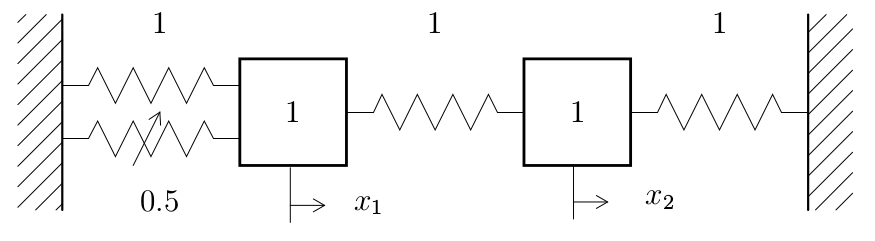
\includegraphics[width=0.7\textwidth]{nnm/2dof_system}
  \caption{Schematic representation of the 2DOF system}
  \label{fig:2dof_system}
\end{figure}

The equations of motion (EOM) are given by

\begin{equation}
  \label{eq:2dof_nonlin_sys}
  \begin{aligned}
    \ddot x_1 + (2x_1 - x_2) + 0.5 x_1^3 &= 0 \\
    \ddot x_2 + (2x_2 - x_2) &= 0
  \end{aligned}
\end{equation}

Note that this system is not symmetric so it possess only non-similar NNMs.


The underlaying linear system is given by

\begin{equation}
  \label{eq:2dof_lin_sys}
  \begin{aligned}
    \ddot x_1 + (2x_1 - x_2) &= 0 \\
    \ddot x_2 + (2x_2 - x_2) &= 0
  \end{aligned}
\end{equation}

The initial condition that excites the two linear modes of system
\eqref{eq:2dof_lin_sys} is found from the eigensolution, i.e. the two
eigenvectors.


Figure \ref{fig:nonlin_time_series} and \ref{fig:nonlin_nnm_config} shows the
time series and configuration plane for in-phase and out-of-phase NNMs for the
nonlinear system. The system vibrates in unison, even though higher harmonics
are present as seen by the curved modal lines in the configuration plot.


\begin{figure}[!ht]
  \centering
  \begin{subfigure}[b]{0.45\textwidth}
    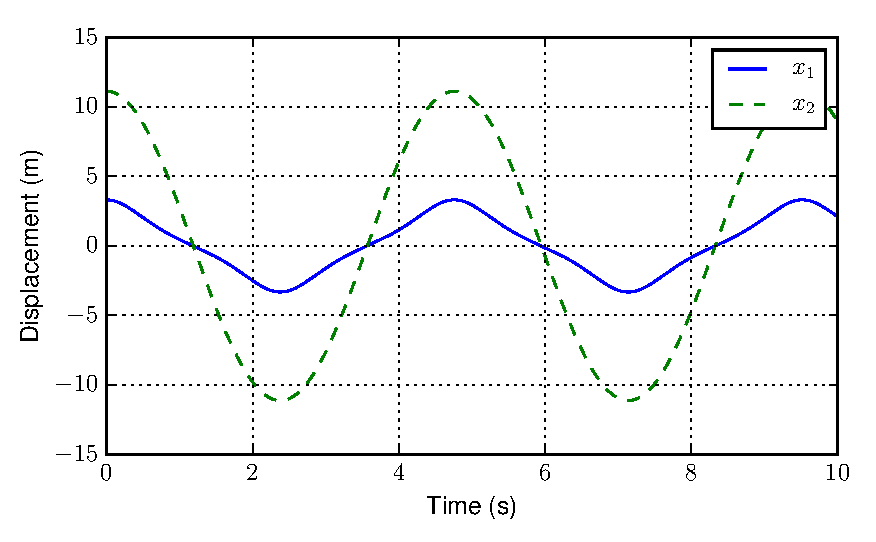
\includegraphics[width=\textwidth]{nnm/nonlin_inphase_time_hist}
  \end{subfigure}
  ~
  \begin{subfigure}[b]{0.45\textwidth}
    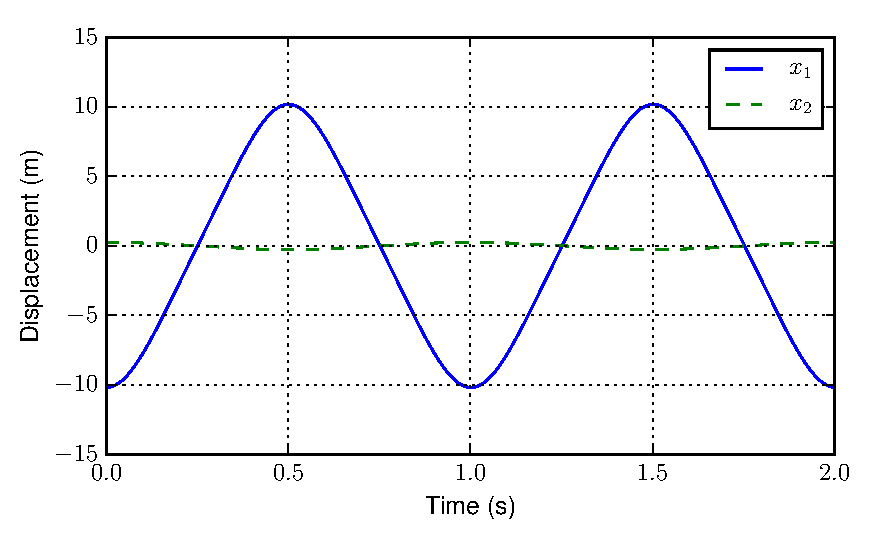
\includegraphics[width=\textwidth]{nnm/nonlin_outphase_time_hist}
  \end{subfigure}
  \caption{Time series of system (\ref{eq:2dof_nonlin_sys}).
    Left plot: in-phase NNM,
    $[x_1(0), x_2(0), \dot x_1(0), \dot x_2(0)] = [3.319, 11.134,0,0]$;
    Right plot: out-of-phase NNM,
    $[x_1(0), x_2(0), \dot x_1(0), \dot x_2(0)] = [-10.188, 0.262,0,0]$.}
  \label{fig:nonlin_time_series}
\end{figure}

\begin{figure}[!ht]
  \centering
  \begin{subfigure}[b]{0.45\textwidth}
    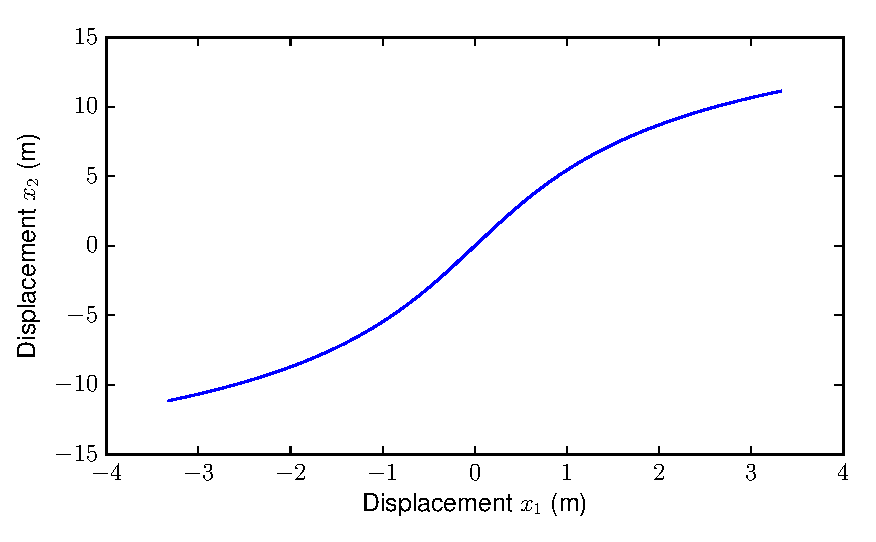
\includegraphics[width=\textwidth]{nnm/nonlin_inphase_conf_space}
  \end{subfigure}
  ~
  \begin{subfigure}[b]{0.45\textwidth}
    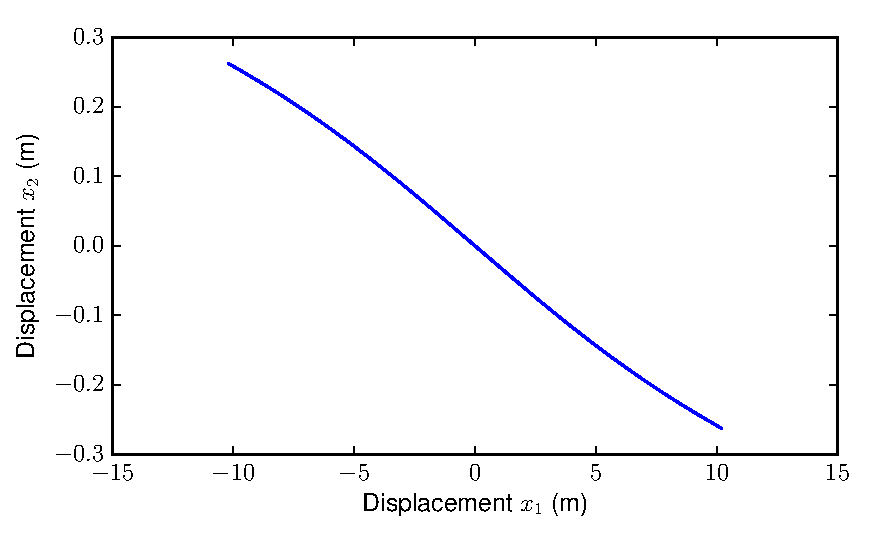
\includegraphics[width=\textwidth]{nnm/nonlin_outphase_conf_space}
  \end{subfigure}
  \caption{NNM motion of system (\ref{eq:2dof_nonlin_sys}) in configuration space.
    Left plot: in-phase NNM;
    Right plot: of-phase NNM.}
  \label{fig:nonlin_nnm_config}
\end{figure}



Figure \ref{fig:nonlin_3:1_int_resonance} shows internal 3:1 resonance. The
motion is still periodic, but not unison.

\begin{figure}[!ht]
  \centering
  \begin{subfigure}[b]{0.45\textwidth}
    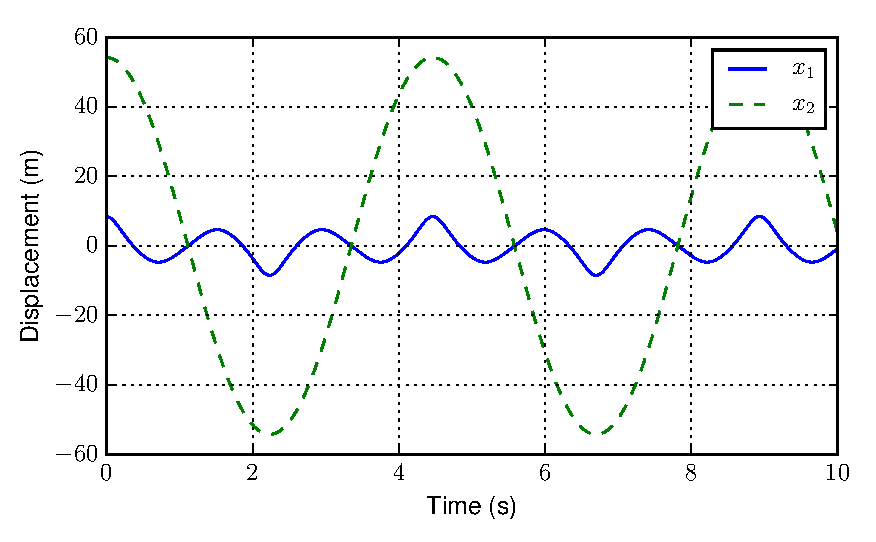
\includegraphics[width=\textwidth]{nnm/nonlin_31_time_hist}
  \end{subfigure}
  ~
  \begin{subfigure}[b]{0.45\textwidth}
    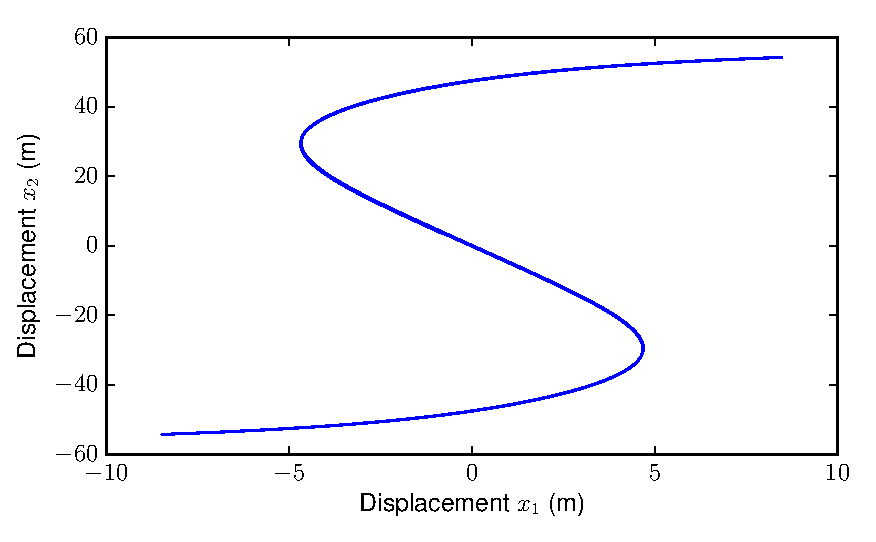
\includegraphics[width=\textwidth]{nnm/nonlin_31_conf_space}
  \end{subfigure}
  \caption{Internally resonant NNM of system \eqref{eq:2dof_nonlin_sys} (3:1
    resonance);
    $[x_1(0), x_2(0), \dot x_1(0), \dot x_2(0)] = [8.476, 54.263, 0, 0]$;
    Left plot: time series;
    Right plot: configuration space}
  \label{fig:nonlin_3:1_int_resonance}
\end{figure}




\subsection{Similar NNM, an example}
\label{sec:similar-nnm-an}


An example of similar NNMs are given in \citep{vakakis1992a}.
Given the symmetric system

\begin{align}
    \ddot x_1 + k_3(x_1 - x_2)^3 + x_1 + x_1^3&= 0 \nonumber \\
    \ddot x_2 - k_3(x_2 - x_2)^3 + x_2 + x_2^3&= 0 \label{eq:2dof_similar_sys}
\end{align}
where $k_3$ is the strength of the nonlinear coupling.
This system possesses only similar NNMs (due to the symmetry), which are found
by imposing the functional relationship

\begin{equation}
  \label{eq:nnm_similar_relation}
  x_2 = c x_1
\end{equation}

where $c \in \Re$ is a real modal constant. Substituting
\eqref{eq:nnm_similar_relation} into \eqref{eq:2dof_similar_sys} to get a
algebraic equation satisfied by the modal constant

\begin{equation}
  \label{eq:nmm_similar_modal}
  k_3(1+c)(c-1)^3 = c(1-c^2)
\end{equation}

From figure \ref{fig:nnm_similar_bifur} it is seen that the system always
possesses the NNMs $x_2 = \pm x_1$ regardless of the coupling strength. This
correspond to the in-phase and out-of-phase similar NNMs respectively and can
be regarded as as a continuation of the two normal modes of the corresponding
linear system.


\begin{figure}[!ht]
  \centering
  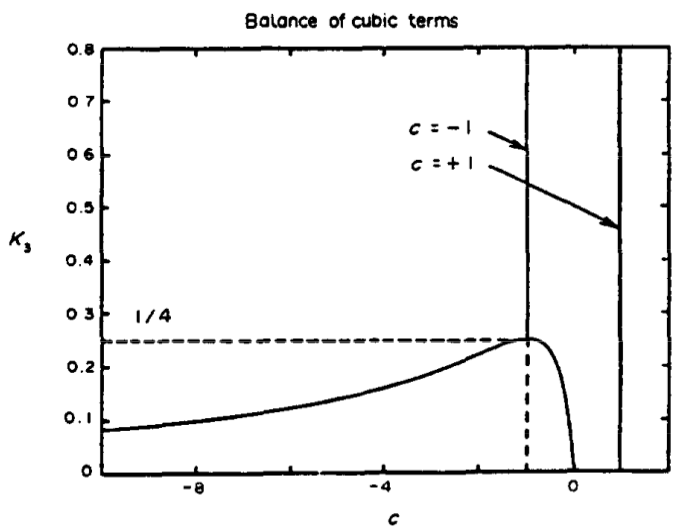
\includegraphics[width=0.7\textwidth]{nnm/similar-nnm-bifur}
  \caption{Pichfork bifurcation of NMMs. (---) stable mode, (- - -) unstable
    mode. From \citep{vakakis1992a}}
  \label{fig:nnm_similar_bifur}
\end{figure}


However at $k_3 = 1/4$, the out-of-phase NNM bifurcates. The bifurcating NNMs are
out-of-phase, time-periodic motions of system and becomes strongly localized as
$k_3 \to 0$, i.e. one node vibrates strongly while the other stands still. This
shows another concept of NNM which differs from LNM: NNMs of a dynamical system
may exceed in number its degrees of freedom. Additionally, NNM bifurcations may
result in mode instability.


Figure \ref{fig:similar_time_series} shows the time series for out-of-phase NNMs
for \eqref{eq:2dof_similar_sys}, and figure \ref{fig:similar_nnm_config} shows
the corresponding configuration space. For the bifurcated NNM, localization is
seen. The system still vibrates with a single harmonic in unison, as seen by the
straight line in configuration space and the time series.

\begin{figure}[!ht]
  \centering
  \begin{subfigure}[b]{0.45\textwidth}
    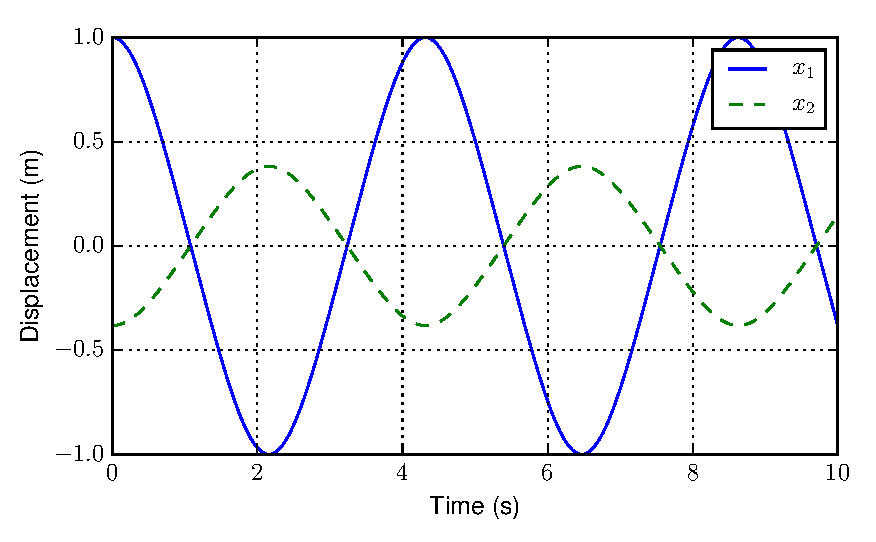
\includegraphics[width=\textwidth]{nnm/similar1_time_hist}
  \end{subfigure}
  ~
  \begin{subfigure}[b]{0.45\textwidth}
    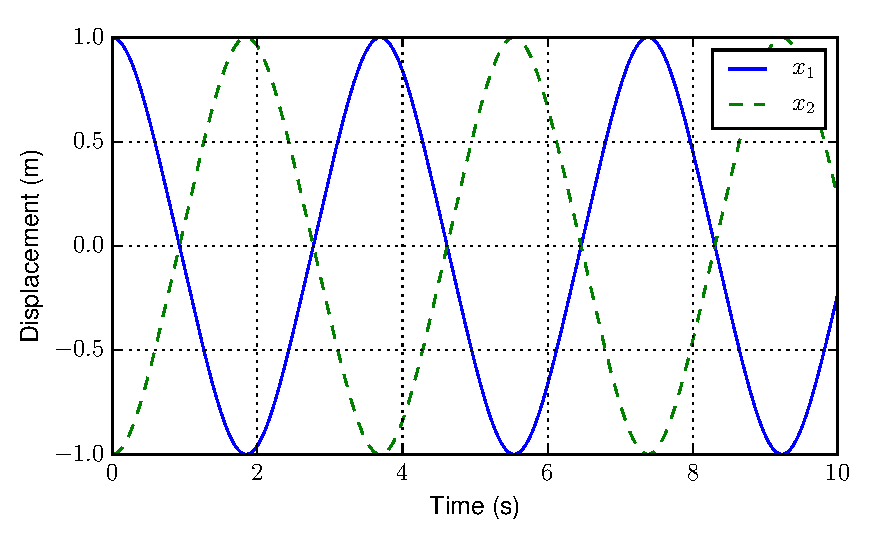
\includegraphics[width=\textwidth]{nnm/similar2_time_hist}
  \end{subfigure}
  \caption{Time series of system \eqref{eq:2dof_similar_sys}.
    Left plot: out-of-phase NNM, $k_3=0.2$,
    $[x_1(0), x_2(0), \dot x_1(0), \dot x_2(0)] = [1,-1,0,0]$;
    Right plot: out-of-phase NNM, $k_3=0.2$,
    $[x_1(0), x_2(0), \dot x_1(0), \dot x_2(0)] = [1, -0.3820,0,0]$.}
  \label{fig:similar_time_series}
\end{figure}


\begin{figure}[!ht]
  \centering
  \begin{subfigure}[b]{0.45\textwidth}
    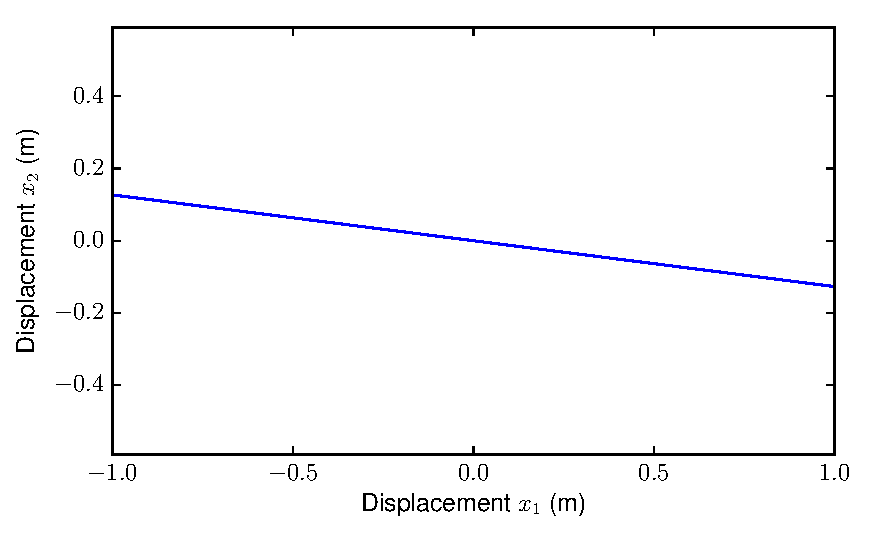
\includegraphics[width=\textwidth]{nnm/similar1_conf_space}
  \end{subfigure}
  ~
  \begin{subfigure}[b]{0.45\textwidth}
    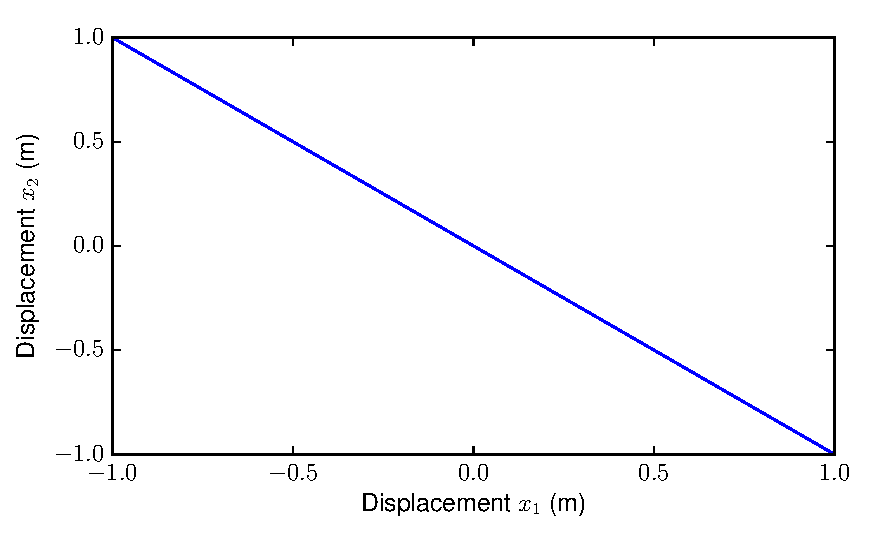
\includegraphics[width=\textwidth]{nnm/similar2_conf_space}
  \end{subfigure}
  \caption{NNM motion of system \eqref{eq:2dof_similar_sys} in configuration space.
    Left plot: out-phase NNM;
    Right plot: out-of-phase NNM.}
  \label{fig:similar_nnm_config}
\end{figure}


%%% Local Variables:
%%% mode: latex
%%% TeX-master: "../../report"
%%% End:
